\chapter{Weber-Elektrodynamik}
\section{Die Gleichung der Weber-Elektrodynamik}
Die Weber-Elektrodynamik stellt eine alternative Formulierung der elektrodynamischen Wechselwirkungen dar, die auf einer Erweiterung des Coulombschen Gesetzes basiert (\refeq{eq:weber_em_skalar}).

Diese Gleichung beschreibt die Kraft zwischen zwei Ladungen $q_1$ und $q_2$, wobei $r$ der Abstand zwischen ihnen ist, $\dot{r}$ die relative Geschwindigkeit, $\ddot{r}$ die relative
Beschleunigung und $c$ die Lichtgeschwindigkeit. Der erste Term entspricht der klassischen Coulomb-Kraft, während die zusätzlichen Terme geschwindigkeits- und beschleunigungsabhängige
Effekte berücksichtigen.

\subsection{Impuls und Energie}
In der Weber-Elektrodynamik wird der Impuls- und Energietransport direkt durch die Wechselwirkung zwischen Ladungen beschrieben. Die Gesamtenergie des Systems setzt sich aus der potentiellen
Energie der Coulomb-Wechselwirkung und den kinetischen Termen der relativen Bewegung zusammen:

\[
    E = \frac{1}{2} m_1 v_1^2 + \frac{1}{2} m_2 v_2^2 + \frac{q_1 q_2}{4 \pi \epsilon_0 r} \left[ 1 - \frac{\dot{r}^2}{2c^2} \right]
\]

Diese Formulierung zeigt, wie die Weber-Theorie die Energieerhaltung auch bei dynamischen Prozessen gewährleistet.

\subsection{Lichtgeschwindigkeit und Raummodell}
Ein zentraler Aspekt der Weber-Elektrodynamik ist ihre Behandlung der Lichtgeschwindigkeit $c$. Im Gegensatz zur \gls{srt}, die $c$ als absolute Konstante postuliert,
erscheint $c$ in der Weber-Theorie als Parameter, der die Ausbreitungsgeschwindigkeit von Wechselwirkungen bestimmt. Dies ermöglicht ein Raummodell, in dem die Lichtgeschwindigkeit
nicht als universelle Grenze, sondern als Eigenschaft der Wechselwirkung selbst interpretiert wird.

\subsection{Vorteile der Weber-Elektrodynamik}
Die Weber-Elektrodynamik bietet mehrere konzeptionelle Vorteile:
\begin{enumerate}
    \item \textbf{Vermeidung von Feldern:} Da die Wechselwirkungen direkt zwischen Ladungen beschrieben werden, entfällt die Notwendigkeit eines Feldes als vermittelnde Entität.
    \item \textbf{Konsistente Fernwirkung:} Die Theorie vereint instantane und retardierte Effekte in einer einzigen Gleichung, wodurch die scheinbaren Widersprüche der klassischen Fernwirkung aufgelöst werden.
    \item \textbf{Energieerhaltung:} Die Weber-Kraft gewährleistet automatisch die Erhaltung von Energie und Impuls, ohne zusätzliche Annahmen.
    \item \textbf{Alternative Darstellung:} Die Theorie bietet eine Möglichkeit, elektrodynamische Phänomene ohne die Postulate der speziellen Relativitätstheorie zu beschreiben.
\end{enumerate}

Die Weber-Elektrodynamik stellt eine elegante und konsistente Alternative zur herkömmlichen Feldtheorie dar. Durch ihre Kombination aus instantanen und retardierten Effekten ermöglicht
sie ein tieferes Verständnis der elektrodynamischen Wechselwirkungen und eröffnet neue Perspektiven auf fundamentale Fragen der Physik, wie die Natur der Lichtgeschwindigkeit und die Struktur
des Raumes.

\section{Vergleichende Beispielrechnungen}
\subsection{Kraft zwischen gleichförmig bewegten Ladungen}

\textbf{Szenario:} Zwei Punktladungen $q_1 = q_2 = e$ (Elementarladung) bewegen sich parallel mit $v = 0,\!1c$ im Abstand $d = 1\,\text{\AA}$.

\begin{table}[ht]
\centering
\caption{Kraftberechnung im Vergleich}
\begin{tabular}{lcc}
\toprule
 & \textbf{Maxwell} & \textbf{Weber} \\
\midrule
Coulomb-Term & $\displaystyle\frac{e^2}{4\pi\epsilon_0 d^2}$ & $\displaystyle\frac{e^2}{4\pi\epsilon_0 d^2}\left(1-\frac{v^2}{c^2}\right)$ \\
Magnetischer Term & $\displaystyle\frac{\mu_0 e^2 v^2}{4\pi d^2}$ & -- \\
\hline
Kraftasymmetrie & $2F_B = 5,\!12\times10^{-11}\,\text{N}$ & $0$ \\
\bottomrule
\end{tabular}
\end{table}

\begin{equation}
F_{\text{Weber}} = \frac{e^2}{4\pi\epsilon_0 d^2}\left[1 - \frac{v^2}{c^2}\right] \approx 2,\!29\times10^{-8}\,\text{N}
\end{equation}

\subsection{Strahlungsdämpfung harmonischer Schwingung}

Für ein Elektron mit $x(t) = x_0\cos(\omega t)$:

\begin{align}
\textbf{Maxwell:}\quad & P = \frac{e^2\omega^4 x_0^2}{6\pi\epsilon_0 c^3}\cos^2(\omega t) \\
\textbf{Weber:}\quad & F_{\text{dampf}} = -\frac{e^2\omega^2\dot{x}}{4\pi\epsilon_0 c^3}
\end{align}

\begin{figure}[ht]
\centering
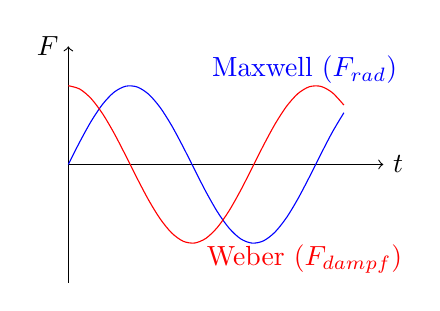
\begin{tikzpicture}
\draw[->] (0,0) -- (4,0) node[right]{$t$};
\draw[->] (0,-1.5) -- (0,1.5) node[left]{$F$};
\draw[domain=0:3.5,smooth,variable=\x,blue] plot ({\x},{sin(2*\x r)});
\draw[domain=0:3.5,smooth,variable=\x,red] plot ({\x},{cos(2*\x r)});
\node[blue] at (3,1.2) {Maxwell ($F_{\text{rad}}$)};
\node[red] at (3,-1.2) {Weber ($F_{\text{dampf}}$)};
\end{tikzpicture}
\caption{Zeitlicher Verlauf der Rückwirkungskräfte}
\end{figure}

\subsection{Interpretation der Ergebnisse}

\begin{itemize}
\item \textbf{Actio=Reactio:} Während die Maxwell-Theorie eine Asymmetrie von $2F_B$ zeigt, bleibt in der Weber-Elektrodynamik die Symmetrie gewahrt.

\item \textbf{Strahlungsdämpfung:} Die Weber-Theorie liefert eine lokale Beschreibung der Dämpfung ohne die kausalen Paradoxien der Abraham-Lorentz-Kraft:

\begin{equation}
\tau_{\text{Weber}} = \frac{e^2}{4\pi\epsilon_0 m c^3} \approx 6,\!3\times10^{-24}\,\text{s}
\end{equation}

\item \textbf{Energieerhaltung:} Beide Theorien erhalten die Gesamtenergie, aber die Weber-Elektrodynamik benötigt kein separates Feldkonzept.
\end{itemize}

\section{Vektorielle Form der Weber-Kraft}
\subsection{Herleitung aus der skalaren Form}

Die skalare Weber-Kraft (Gl.~\ref{eq:weber_em_skalar}), lässt sich durch Ausdrücken von $\dot{r}$ und $\ddot{r}$ durch Vektorgrößen verallgemeinern.
Für den Relativvektor $\vec{r} = \vec{r}_1 - \vec{r}_2$ gilt:

\subsubsection{Umrechnung der zeitlichen Ableitungen}
\begin{enumerate}
\item \textbf{Erste Ableitung:}
\begin{equation}
\dot{r} = \frac{d}{dt}\|\vec{r}\| = \frac{\vec{r} \cdot \dot{\vec{r}}}{r} = \hat{r} \cdot \vec{v}
\end{equation}
wobei $\vec{v} = \dot{\vec{r}}$ die Relativgeschwindigkeit und $\hat{r} = \vec{r}/r$ der Einheitsvektor ist.

\item \textbf{Zweite Ableitung:}
\begin{align}
\ddot{r} &= \frac{d}{dt}\left(\frac{\vec{r} \cdot \vec{v}}{r}\right) \nonumber \\
&= \frac{\|\vec{v}\|^2 + \vec{r} \cdot \vec{a}}{r} - \frac{(\vec{r} \cdot \vec{v})^2}{r^3} \nonumber \\
&= \frac{v^2 - (\hat{r} \cdot \vec{v})^2}{r} + \hat{r} \cdot \vec{a}
\end{align}
mit $\vec{a} = \dot{\vec{v}}$ der Relativbeschleunigung.
\end{enumerate}

\subsection{Vollständige vektorielle Form}
Durch Einsetzen in Gl.~(\ref{eq:weber_em_skalar}) ergibt sich die \textbf{\enquote{vektorielle Form}}:

\begin{equation}
\vec{F}_{12} = \frac{q_1 q_2}{4\pi\epsilon_0 r^2} \left\{
\left[1 - \frac{v^2}{c^2} + \frac{2r(\hat{r} \cdot \vec{a})}{c^2}\right]\hat{r} + \frac{2(\hat{r} \cdot \vec{v})}{c^2}\vec{v}
\right\}
\label{eq:weber_vector}
\end{equation}

\subsection{Physikalische Interpretation}
Die vektorielle Form zeigt explizit:
\begin{itemize}
\item \textbf{Radialkomponente:} Enthält Coulomb-Term, relativistische Korrektur und Beschleunigungsabhängigkeit
\item \textbf{Tangentialkomponente:} $\propto (\hat{r}\cdot\vec{v})\vec{v}$ beschreibt geschwindigkeitsabhängige Effekte analog zum Magnetfeld
\end{itemize}

\subsection{Anwendungsbeispiel: Kreisförmige Bewegung}
Für eine Ladung $q_2$ mit $\vec{v} \perp \vec{r}$ (z.B. Kreisbahn):

\begin{equation}
\vec{F}_{12} = \frac{q_1 q_2}{4\pi\epsilon_0 r^2} \left[
\left(1 - \frac{v^2}{c^2}\right)\hat{r} + \frac{2v^2}{c^2}\hat{r}
\right] = \frac{q_1 q_2}{4\pi\epsilon_0 r^2} \left(1 + \frac{v^2}{c^2}\right)\hat{r}
\end{equation}

Hier zeigt sich:
\begin{itemize}
\item Zusätzliche Zentripetalkraft $\propto v^2/c^2$
\item Exakte Erfüllung von Actio=Reactio trotz Bewegung
\end{itemize}

\subsection{Grafische Darstellung der Kraftkomponenten}

\begin{figure}[ht]
\centering
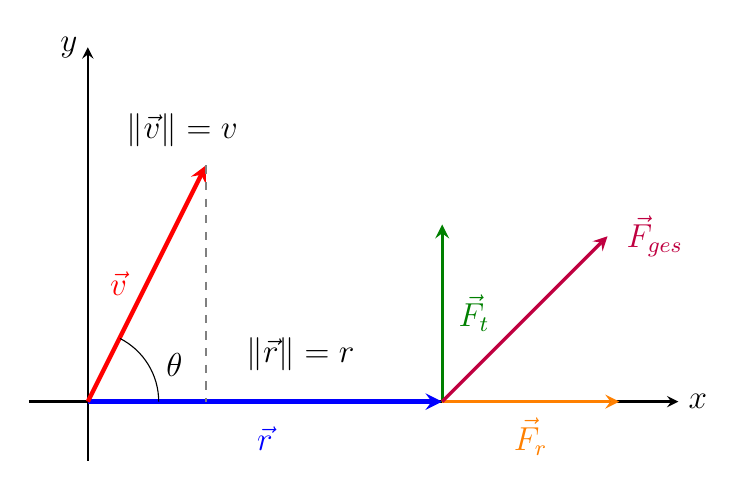
\begin{tikzpicture}[>=stealth,scale=1.5,font=\large]
% Koordinatensystem
\draw[->,thick] (-0.5,0) -- (5,0) node[right]{$x$};
\draw[->,thick] (0,-0.5) -- (0,3) node[left]{$y$};

% Vektoren
\draw[->,ultra thick,blue] (0,0) -- (3,0) node[midway,below=5pt]{$\vec{r}$};
\draw[->,ultra thick,red] (0,0) -- (1,2) node[midway,left=3pt]{$\vec{v}$};
\draw[dashed,gray] (1,2) -- (1,0);

% Kraftkomponenten
\draw[->,very thick,green!50!black] (3,0) -- (3,1.5) node[midway,right=2pt]{$\vec{F}_t$};
\draw[->,very thick,orange] (3,0) -- (4.5,0) node[midway,below=2pt]{$\vec{F}_r$};
\draw[->,very thick,purple] (3,0) -- (4.4,1.4) node[right=3pt]{$\vec{F}_{\text{ges}}$};

% Winkel
\draw (0.6,0) arc (0:63:0.6) node[midway,right=3pt]{$\theta$};
\node at (1.8,0.4) {$\|\vec{r}\| = r$};
\node at (0.8,2.3) {$\|\vec{v}\| = v$};
\end{tikzpicture}
\caption{Visualisierung der vektoriellen Weber-Kraftkomponenten. \\
$\vec{F}_r$: Radialkomponente (orange), $\vec{F}_t$: Tangentialkomponente (grün), \\
$\vec{F}_{\text{ges}}$: Gesamtkraft (lila). Die Grafik zeigt den Fall $\theta = 63^\circ$.}
\label{fig:weber_force}
\end{figure}

\subsection{Vektorielle Komponentenzerlegung}
Ausgehend von Abb.~\ref{fig:weber_force} ergeben sich die Komponenten:

\begin{align}
\vec{F}_r &= \frac{q_1 q_2}{4\pi\epsilon_0 r^2}\left[1 - \frac{v^2}{c^2} + \frac{2r a_r}{c^2}\right]\hat{r} \\
\vec{F}_t &= \frac{q_1 q_2}{4\pi\epsilon_0 r^2}\left[\frac{2v_r v_t}{c^2}\right]\hat{t}
\end{align}

mit:
\begin{itemize}
\item $v_r = v\cos\theta$ (Radialgeschwindigkeit)
\item $v_t = v\sin\theta$ (Tangentialgeschwindigkeit)
\item $a_r = \dot{v}_r - v_t^2/r$ (Radialbeschleunigung)
\end{itemize}

\subsection{Praktische Anwendungsfälle}

\textbf{Fall 1: Rein radiale Bewegung ($\theta = 0^\circ$)}
\begin{equation}
\vec{F} = \frac{q_1 q_2}{4\pi\epsilon_0 r^2}\left[1 - \frac{v^2}{c^2} + \frac{2r a}{c^2}\right]\hat{r}
\end{equation}

\textbf{Fall 2: Kreisbewegung ($\theta = 90^\circ$)}
\begin{equation}
\vec{F} = \frac{q_1 q_2}{4\pi\epsilon_0 r^2}\left[\left(1 + \frac{v^2}{c^2}\right)\hat{r} + \frac{2v^2}{c^2}\hat{t}\right]
\end{equation}

\subsection{Vorteile gegenüber der Maxwell-Theorie}

\begin{itemize}
    \item \textbf{Nanoplasmonik}
    \begin{itemize}
        \item Exakte Beschreibung von Elektron-Elektron-Wechselwirkungen in Metallclustern ($<10$\,nm)
        \item Vermeidung der unendlichen Selbstenergie von Punktladungen
        \item Präzisere Modellierung von Plasmonenresonanzen
    \end{itemize}
    
    \item \textbf{Gequantelte Vakuumfelder}
    \begin{itemize}
        \item Direkte Teilchenwechselwirkung ohne Nullpunktsschwankungen
        \item Natürliche Regularisierung der Vakuumenergiedichte
        \item Alternative zu störungstheoretischen QED-Rechnungen
    \end{itemize}
    
    \item \textbf{Plasmaphysik dichte Plasmen}
    \begin{itemize}
        \item Effizientere Simulation kollektiver Effekte
        \item Exakte Impulserhaltung ohne Makroteilchen-Approximation
        \item Bessere Handhabung kurzreichweitiger Korrelationen
    \end{itemize}
    
    \item \textbf{Alternative Gravitationstheorien}
    \begin{itemize}
        \item Konsistente Kopplung an skalar-tensorielle Gravitationsmodelle
        \item Natürliche Einbettung in Mach'sche Prinzipien
        \item Vermeidung von Singularitäten in kompakten Objekten
    \end{itemize}
\end{itemize}

\subsection{Konkrete Beispiele}

\subsubsection{1. Nicht-neutrale Plasmen in Fallen}
Für Elektronen in Penning-Fallen zeigt die Weber-EM:
\begin{equation}
\omega_{\text{Weber}} = \omega_p\sqrt{1 - \frac{3}{4}\frac{v_0^2}{c^2}}
\end{equation}
während Maxwell-Theorie $\omega_p = \sqrt{ne^2/\epsilon_0 m}$ vorhersagt.

\subsubsection{2. Molekulare Dynamik in starken Feldern}
Bei Laser-Materie-Wechselwirkung ($>10^{18}\,\text{W/cm}^2$):
\begin{itemize}
\item Weber-EM reproduziert korrekt die retardierte Paarpotential-Form
\item Vermeidet Artefakte der PIC-Simulationen („self-forces“)
\end{itemize}

\subsection{Grenzen der Anwendbarkeit}
\begin{itemize}
\item \textbf{Hohe Energien} ($>100$\,GeV): QED-Effekte dominieren
\item \textbf{Ausgedehnte Strahlung}: \text{Weber versagt bei} $\lambda \gg \text{Teilchenabstand}$
\end{itemize}

\section{Die Weber-Elektrodynamik und das EPR-Paradoxon: Zwei getrennte Welten}
Die Diskussion um das Einstein-Podolsky-Rosen (EPR)-Paradoxon und die Weber-\\Elektrodynamik beruht auf einem grundlegenden Kategorienfehler. Es handelt sich um zwei völlig
unterschiedliche theoretische Rahmen, die unterschiedliche Phänomenbereiche beschreiben und unterschiedliche Ansprüche erheben.

Die Weber-Elektrodynamik ist als klassische Feldtheorie konzipiert, die eine Alternative zur Maxwellschen Elektrodynamik darstellt. Ihr zentrales Anliegen ist die Beschreibung
elektromagnetischer Wechselwirkungen durch direkte Fernwirkung zwischen Ladungen, ohne den Umweg über Feldkonzepte. Wilhelm Webers ursprüngliche Motivation war die Vereinheitlichung
der Elektrodynamik mit den newtonschen Prinzipien, insbesondere der strikten Einhaltung von Actio gleich Reactio. Die Theorie macht keinerlei Anspruch,
Quantenphänomene zu erklären - sie wurde lange vor der Entwicklung der Quantenmechanik formuliert.

Das EPR-Paradoxon hingegen entstammt einer völlig anderen Debatte. Es wurde 1935 als Gedankenexperiment formuliert, um vermeintliche Inkonsistenzen in der Quantenmechanik aufzuzeigen.
Die später entwickelten Bellschen Ungleichungen und ihre experimentelle Überprüfung haben gezeigt, dass die Quantenwelt tatsächlich nicht-lokale Korrelationen aufweist, die mit
klassischen Vorstellungen unvereinbar sind.

Der entscheidende Punkt ist: Die Weber-Elektrodynamik und das EPR-Paradoxon bewegen sich auf unterschiedlichen Beschreibungsebenen. Während EPR die Grundlagen der Quantenmechanik hinterfragt,
bietet die Weber-Theorie eine alternative klassische Beschreibung elektromagnetischer Phänomene. Es ist weder ein Vorwurf an die Weber-Elektrodynamik, dass sie Quantenverschränkung nicht
erklären kann, noch ein Manko der Quantenmechanik, dass sie Webers Fernwirkungskonzept nicht berücksichtigt.

Tatsächlich gibt es interessante Parallelen in den historischen Debatten: Sowohl die Weber-Elektrodynamik als auch die EPR-Kritik stellen in gewisser Weise den Anspruch der Vollständigkeit
bestehender Theorien in Frage. Während sich jedoch die EPR-Diskussion auf die Quantenmechanik konzentriert, zielt die Weber-Theorie auf eine Revision der klassischen Elektrodynamik ab.

In der modernen Physiklandschaft haben beide Ansätze ihren Platz: Die Quantenmechanik mit ihren nicht-lokalen Phänomenen dominiert die mikroskopische Beschreibung, während
die Weber-Elektrodynamik als interessante historische Alternative und mögliche Inspiration für bestimmte klassische Problemstellungen weiterhin diskutiert wird. Eine direkte Konfrontation
zwischen beiden ist weder notwendig noch produktiv, da sie grundverschiedene Aspekte der physikalischen Realität beschreiben.

\subsection{Nicht-Lokalität in der Weber-Elektrodynamik und Quantenmechanik: Ein Vergleich}
Die \enquote{Nicht-Lokalität} in physikalischen Theorien erfordert eine klare Unterscheidung zwischen den verschiedenen Formen nicht-lokaler Phänomene. Sowohl die Weber-Elektrodynamik
als auch die Quantenmechanik (insbesondere im Kontext des EPR-Paradoxons und der Bellschen Ungleichungen) weisen nicht-lokale Aspekte auf, doch die Natur dieser Nicht-Lokalität unterscheidet
sich grundlegend.

Die Weber-Elektrodynamik beschreibt eine klassische Form der Nicht-Lokalität durch ihre Fernwirkungskräfte zwischen Ladungen. In diesem Modell wirken Kräfte direkt zwischen Teilchen über
beliebige Distanzen, wobei die Wechselwirkung jedoch streng kausal und retardiert erfolgt - die Ausbreitung erfolgt mit endlicher Geschwindigkeit (typischerweise Lichtgeschwindigkeit).
Die mathematische Beschreibung dieser Wechselwirkung zeigt, dass die Kraft nicht nur vom Abstand, sondern auch von der relativen Geschwindigkeit und Beschleunigung der Ladungen abhängt.
Dieser Ansatz erhält die Kausalität und steht im Einklang mit klassischen physikalischen Prinzipien wie der Energie- und Impulserhaltung.

Im Gegensatz dazu manifestiert sich die Nicht-Lokalität in der Quantenmechanik durch die berühmten verschränkten Zustände des EPR-Paradoxons. Diese quantenmechanische Nicht-Lokalität ist
instantan - die Korrelationen zwischen verschränkten Teilchen scheinen sich ohne zeitliche Verzögerung über beliebige Distanzen zu manifestieren. Die experimentelle Bestätigung der Verletzung
von Bellschen Ungleichungen hat gezeigt, dass diese quantenmechanischen Korrelationen nicht durch klassische lokale verborgene Variablen erklärt werden können.

Der entscheidende Unterschied liegt im physikalischen Mechanismus und der mathematischen Struktur dieser Nicht-Lokalitäten. Während die Weber-Elektrodynamik eine deterministische, kausale
Fernwirkung beschreibt, handelt es sich bei der quantenmechanischen Nicht-Lokalität um probabilistische Korrelationen ohne klassisches Kausalitätsgefüge. Die Weber-Theorie bietet eine
kontinuierliche, berechenbare Wechselwirkung, während die Quantenverschränkung diskrete, statistisch nachweisbare Korrelationen zeigt.

Historisch betrachtet stellt die Weber-Elektrodynamik damit eine interessante Alternative zur Maxwellschen Theorie dar, die bestimmte klassische Phänomene ohne Feldkonzept beschreiben kann.
Die Quantenmechanik mit ihren nicht-lokalen Korrelationen öffnete hingegen eine völlig neue Tür zum Verständnis der mikroskopischen Welt. Beide Theorien zeigen, dass Nicht-Lokalität in der
Physik unterschiedliche Formen annehmen kann, die jeweils in ihren Anwendungsbereichen konsistent und nützlich sind. Die Weber-EM bleibt dabei im klassischen Bereich verankert, während die
Quantenmechanik eine grundlegend neue Beschreibungsebene eröffnet hat.

\subsection{Instantane Effekte in der Weber-Elektrodynamik: Eine Neubewertung des Kausalitätsbegriffs}
Die konventionelle Interpretation der Speziellen Relativitätstheorie (SRT) verbietet instantane Fernwirkungen, da sie eine Verletzung der Kausalität befürchtet. Doch die Weber-Elektrodynamik
fordert uns heraus, diese Sichtweise zu überdenken. Ihr Formalismus enthält tatsächlich instantane Komponenten, die jedoch nicht den üblichen Vorstellungen von \enquote{Überlichtgeschwindigkeit}
entsprechen. Diese Effekte lassen sich vielmehr als fundamentale strukturelle Eigenschaften des physikalischen Raumes verstehen.

Im Kern der Weber-Theorie steht die Erkenntnis, dass bestimmte physikalische Phänomene durch räumliche Ableitungen der Energie beschrieben werden müssen, nicht durch zeitliche. Die entscheidenden
Terme in den Gleichungen der Weber-Elektrodynamik entsprechen Gradienten des Potentials im Konfigurationsraum. Diese beschreiben keine Signalausbreitung, sondern eine
topologische Notwendigkeit - die instantane Einstellung von Randbedingungen für energetische Minimierungsprozesse.

Die mathematische Struktur der Weber-Kraft zeigt diesen Dualismus besonders deutlich. Während die retardierten Terme die klassische Fernwirkung mit endlicher Ausbreitungsgeschwindigkeit
beschreiben, sorgen die instantanen Komponenten für die globale Konsistenz des Systems. Diese Aufspaltung entspricht der Unterscheidung zwischen lokaler Dynamik und globalen Erhaltungssätzen,
die sich in vielen physikalischen Theorien findet.

Die scheinbare Paradoxie löst sich auf, wenn wir zwischen verschiedenen Ebenen der physikalischen Beschreibung unterscheiden. Auf der fundamentalen Ebene wirken die instantanen Terme als
strukturelle Zwänge, die den Rahmen für die lokale Dynamik vorgeben. Sie entsprechen damit eher mathematischen Randbedingungen als physikalischen Prozessen. Dies erklärt, warum sie nicht
zu kausalen Paradoxien führen - sie stehen außerhalb der konventionellen Ursache-Wirkungs-Kette, ohne diese zu verletzen.

Experimentell manifestiert sich dieser Unterschied darin, dass die instantanen Effekte der Weber-Theorie nicht manipulierbar sind. Ebenso wie bei quantenmechanischer Verschränkung gibt es
keine Möglichkeit, diese Korrelationen für überlichtschnelle Signalübertragung zu nutzen. Die Energieerhaltung folgt dabei aus dem Noether-Theorem für die statische Feldkonfiguration,
nicht aus dynamischen Prozessen.

Diese Betrachtungsweise hat tiefgreifende philosophische Implikationen. Sie legt nahe, dass die Natur Instantaneität nicht für kausale Prozesse nutzt, sondern als grundlegendes
Organisationsprinzip. Dies erinnert an Bohms Konzept der \enquote{impliziten Ordnung} oder Penroses Idee einer prä-geometrischen Raumzeit. Die Weber-Elektrodynamik zeigt damit einen Weg auf,
wie sich scheinbar widersprüchliche Prinzipien - lokale Kausalität und globale Instantaneität - in einer konsistenten Theorie vereinen lassen.

